\chapter{Problem Formulation and System Overview}
\label{chap:faire_overview}

\section{A Local Motion--Force Task}
The task formulation connects a spatial instruction to a physical operation. A region identifies the intended working area, while a skill supplies the temporally related references needed to approach, traverse under load, and exit. Keeping these descriptions separate makes it possible to compare different skill providers without changing the meaning of the task.

Let \(\Omega\subset\R^2\) denote the selected local region in the robot-base XY plane and let \(c=[c_x,c_y]^\mathsf{T}\) be a frozen task origin in millimeters. The region is specified by a person through the physical marking or the experiment's region parameters. A registered RGB image \(I_k\), tool pose \(q_k=[p_k^\mathsf{T},\rho_k^\mathsf{T}]^\mathsf{T}\), and measured force \(f_k^{\mathrm{meas}}\) describe the available execution context. Orientation is stored as a rotation vector in radians. The action representation is
\begin{equation}
 a_{k+j}=\begin{bmatrix}p_{k+j}^{\mathrm{ref}}\\\rho_{k+j}^{\mathrm{ref}}\\f_{k+j}^{\mathrm{target}}\end{bmatrix}\in\R^9,
 \qquad j=0,\ldots,H-1.
 \label{eq:motion_force_prediction}
\end{equation}
The reference does not directly command joint torque. It describes a future pose and target force for the execution system. The learned pose-only condition uses the first six components and obtains its force reference externally.

A \emph{local polishing skill} is the sequence \(A_k=(a_k,\ldots,a_{k+H-1})\), together with its physical sample timing and the task registration used to restore absolute coordinates. Pairing movement and force in this sequence represents when a target load accompanies a location or motion phase. It does not imply that the robot will realize the exact demonstrated velocity or force at every instant. Those quantities also depend on command conditioning, controller dynamics, and the physical contact.

\section{Human Guidance and the Region Interface}
Human guidance contributes both a spatial specification and examples of temporal behavior. The visible mark gives a practical cue for the local operation. The region-registration implementation can detect a dark marked region within a calibrated image area, map it to the working plane, and freeze its center and principal-axis direction. Figure~\ref{fig:mark_example} illustrates that interface using a genuine archived camera image.

\begin{figure}[tbp]\centering
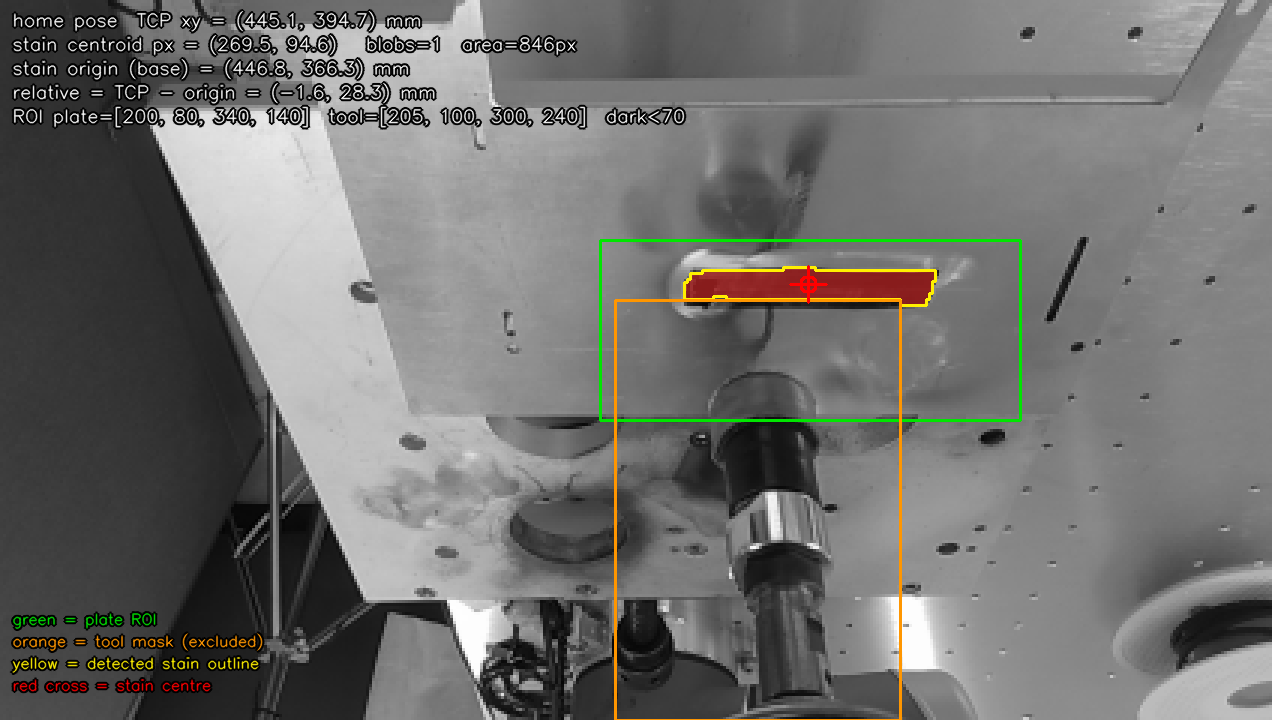
\includegraphics[width=0.87\linewidth]{figures/mark_detection_example.png}
\caption[Marked local region and registration]{Archived camera view of a marked local region and its registration overlay. The colored outlines belong to the existing detection display. This is an example of spatial instruction and image registration, not a validated micro-scratch detector or the fixed-origin E1 trial image.}
\label{fig:mark_example}
\end{figure}

The evaluated E1 comparison fixes \(c=(457.4,375.0)\) mm for all providers. Its evaluation band is specified independently by endpoints and width. The origin is a registration datum; it need not coincide with the midpoint of that band. In E2, the existing per-run origin interface is retained. Neither experiment uses a height-condition label as a policy input.

The policy's external stain-mask option is disabled for the evaluated checkpoints. Instead, the image encoder derives a fixed TCP interaction-region feature from RGB. The physical marking, the registered origin, the evaluator's spatial band, and the encoder's image ROI are therefore four different objects. Conflating them would incorrectly imply that the network is explicitly constrained to the evaluator's band or that it receives a segmentation of the complete processing strategy.

\section{Module Responsibilities}
Figure~\ref{fig:faire_architecture} shows the implemented path from human guidance to evaluation. A provider supplies a sequence, a common execution layer converts it into conditioned commands, and the lower-level controller produces the physical interaction. Measured robot pose and force provide feedback. Evaluation observes this interaction through its own procedural criteria.

\begin{figure}[tbp]\centering
\resizebox{\linewidth}{!}{%
\begin{tikzpicture}[node distance=8mm]
\node[block,text width=42mm] (human) {Human region specification\\mark / fixed task origin};
\node[block,text width=42mm,right=12mm of human] (teach) {Motion--force teaching\\RGB, pose, force, time};
\node[block,text width=42mm,below=of human] (registration) {Task registration\\center; optional axis alignment};
\node[block,text width=42mm,below=of teach] (learning) {Dataset and policy learning\\conditional Flow Matching};
\node[block,text width=96mm,below=10mm of $(registration.south)!0.5!(learning.south)$] (provider) {Action provider: rules R / teaching replay T / policy C\\time-related pose and target-force sequence};
\node[block,text width=96mm,below=of provider] (exec) {Shared executor and pose conditioner\\coordinate restoration, plan connection, command limits};
\node[block,text width=96mm,below=of exec] (control) {Existing force controller and robot\\contact regulation; measured pose and force};
\node[block,text width=96mm,below=of control] (eval) {Contact-task evaluator / recorded analysis\\contact, ordered loaded pass, unload and rise};
\draw[link] (human)--(registration);\draw[link] (teach)--(learning);
\draw[link] (registration.south)--(provider.north west);
\draw[link] (learning.south)--(provider.north east);
\draw[link] (provider)--(exec);\draw[link] (exec)--(control);\draw[link] (control)--(eval);
\draw[link] (control.east)--++(9mm,0)|- (provider.east);
\node[rotate=90,font=\scriptsize,fill=white,inner sep=2pt]
 at ($(control.east)+(9mm,17mm)$) {measured observations};
\draw[link,dashed] (eval.west)--++(-9mm,0)|- (exec.west);
\node[rotate=90,font=\scriptsize,fill=white,inner sep=2pt]
 at ($(eval.west)+(-9mm,15mm)$) {completion finish};
\end{tikzpicture}}
\caption[System overview and module interfaces]{Implemented system overview. Solid arrows show data or execution flow. The dashed arrow requests the existing finish/hold after procedural completion; it does not synthesize an exit motion. The diagram is conceptual and editable. E2 uses its separate operator-terminated protocol.}
\label{fig:faire_architecture}
\end{figure}

\begin{table}[tbp]\centering\small
\caption[Module responsibilities]{Responsibilities of the human and system components.}
\label{tab:module_responsibilities}
\begin{tabularx}{\textwidth}{P{0.24\textwidth}X}
\toprule Component & Responsibility \\ \midrule
Human operator & Specify the local task, demonstrate motion and loading, set up the specimen, and provide recorded field observations. \\
Teaching system & Register tracked tool pose and record paired RGB, pose, force, and receipt-time evidence. \\
Skill provider & Supply a time-related reference sequence using a rule, a fixed demonstration, or a conditioned generator. \\
Common executor & Restore coordinates, interpolate references, connect plans, condition commands, and manage the existing finish/hold procedure. \\
Lower-level controller & Regulate physical contact using the supplied target force and measured state. \\
Task evaluator & Recognize the defined contact procedure and report its outcome; it does not measure surface quality. \\
\bottomrule
\end{tabularx}
\end{table}

\section{Physical Platform and Observations}
The robot interface is the UR10 system identified by the deployed \texttt{ur10skku} topics and Cartesian command services. The teaching side uses a Vive tracker, calibrated tool pose, force/torque sensing, and a RealSense RGB stream. Robot execution records TCP pose from robot feedback and a processed six-axis wrench. The policy uses only the three force components. Torques remain useful logged diagnostics but are not policy inputs or actions for these checkpoints.

\begin{figure}[tbp]\centering
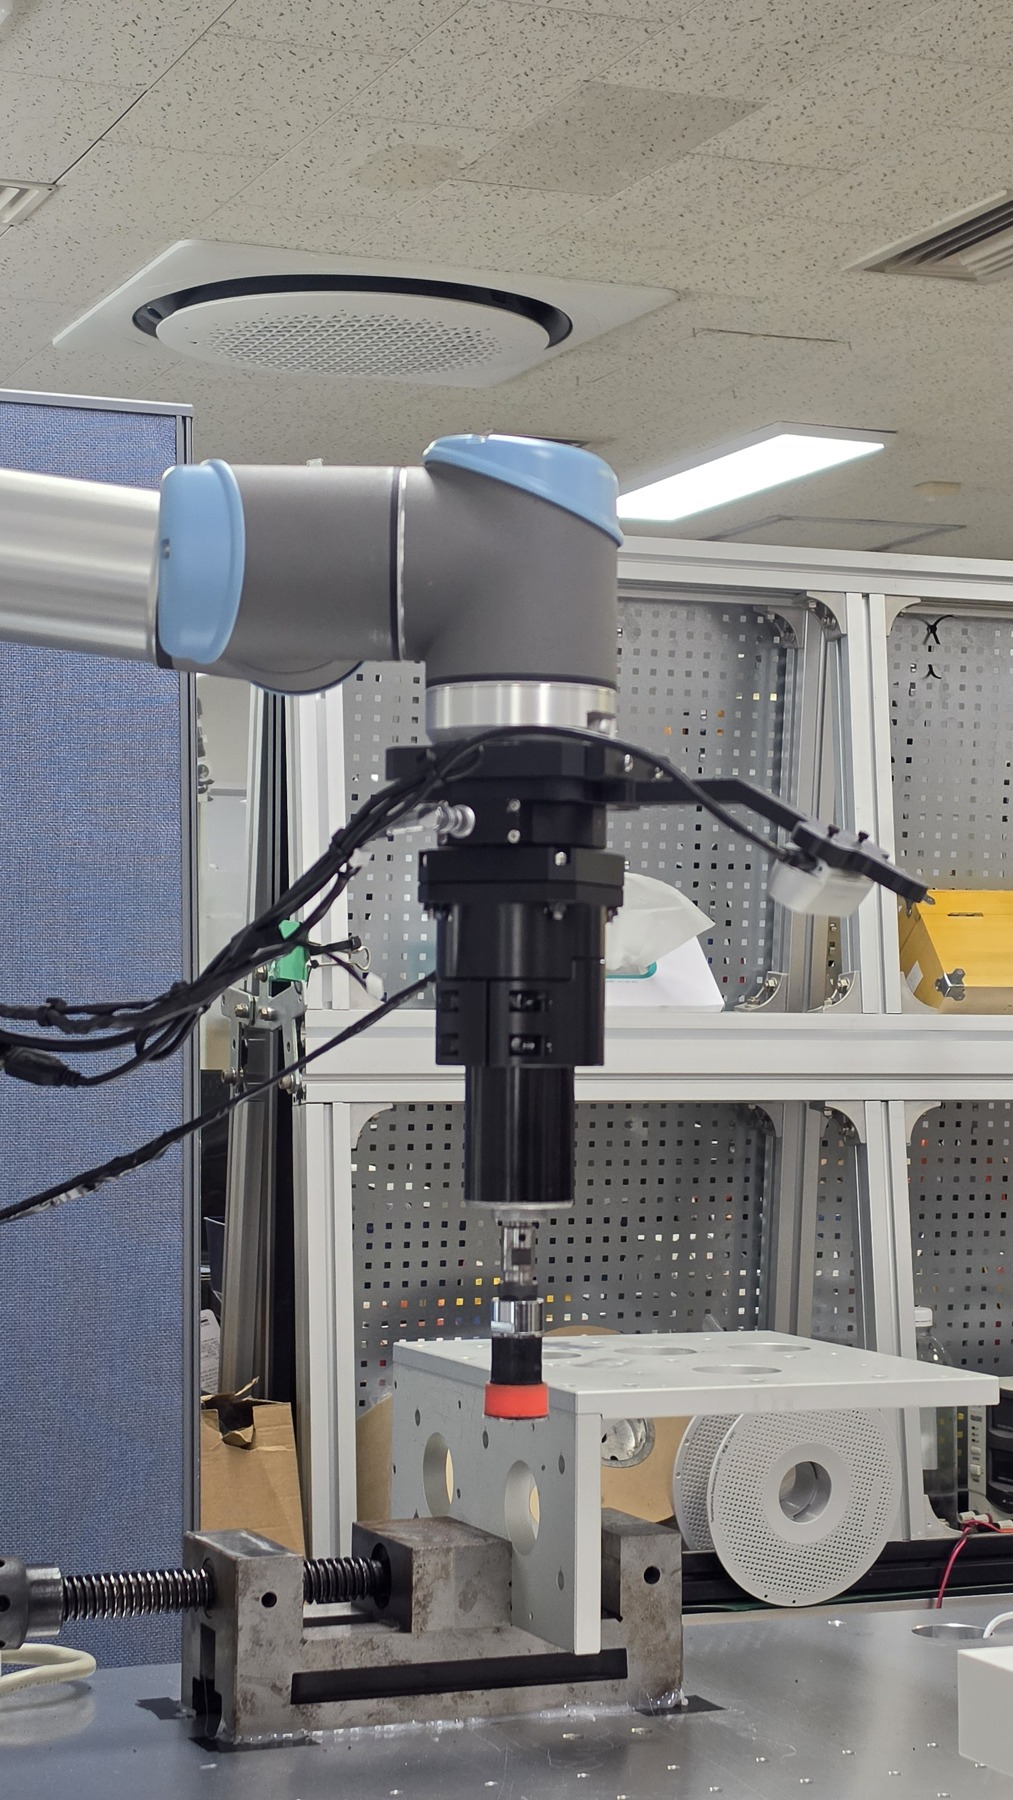
\includegraphics[width=0.67\linewidth,height=0.49\textheight,keepaspectratio]{figures/apparatus_20260807.jpg}
\caption[Archived robot apparatus photograph]{Genuine archived apparatus photograph dated 7 August 2026, showing the robot-mounted processing tool and fixture. Only image rotation and proportional resizing were applied. It illustrates the local experimental platform; it is not presented as a photograph taken during the October E1 or E2 runs.}
\label{fig:apparatus}
\end{figure}

The available records support a description of a robot-mounted local processing tool acting on a marked plate. They do not specify a complete process qualification, including measured spindle speed, material alloy, abrasive grade, or pre/post roughness. The experiments therefore use the measured robot interaction to answer procedural questions. These limits do not prevent reproducing the learning and execution interfaces, but they restrict claims about manufacturing outcomes.

\section{Stain-Centered Learning and Direction Transfer}
\label{sec:stain_relative_generalization}
The representation separates the local movement pattern from its placement on the plate. Its training-data transformation expresses observation and action positions relative to a frozen stain center:
\begin{equation}
 \widetilde p_k=[p_{k,x}-c_x,\ p_{k,y}-c_y,\ p_{k,z}]^\mathsf{T},
 \qquad \widetilde\rho_k=\rho_k.
 \label{eq:relative_task_pose}
\end{equation}
This transformation retains the base-axis orientation and absolute Z coordinate. A single-direction demonstration consequently teaches a center-relative movement pattern in its original reference direction. The implementation additionally supports transferring that learned pattern to another in-plane stain direction through coordinated observation and action transformations. Training on centered positions and aligning directions at inference are two connected parts of the transfer mechanism; the dataset converter itself does not rotate the training episodes.

\subsection{Center and Axis from the Specified Region}
The reference-free registration path detects dark pixels within a configured plate area, excludes the tool area, and maps the retained pixels to robot-base XY coordinates using each image's pose-dependent planar homography. It pools these mapped points across the registration frames. Starting from their coordinate-wise median, four iterations retain the nearest 85\% of points and update the center by their mean. A singular-value decomposition of the trimmed, centered point cloud supplies the dominant strip axis. Its angle \(\theta_{\mathrm{live}}\in[0,\pi)\) is measured in base-plane radians. The axis is unoriented: the same strip has directions differing by \(\pi\), rather than an identified stroke-start endpoint.

The resulting center and optional angle are frozen together for the episode. An operator-supplied live angle is also supported. The direction therefore enters through explicit task registration rather than a learned output head. A center recovered from the visible mark identifies the intended task; it does not estimate defect depth or determine the desired force schedule.

\subsection{Observation Alignment and Path Restoration}
Let \(\theta_{\mathrm{ref}}\) denote the base-plane axis associated with the teaching reference direction. The implemented alignment angle and planar rotation are
\begin{align}
 \alpha&=\operatorname{wrap}_{\pi}
       (\theta_{\mathrm{ref}}-\theta_{\mathrm{live}}),
 &\operatorname{wrap}_{\pi}(\delta)
   &=((\delta+\pi/2)\bmod\pi)-\pi/2,\label{eq:stain_axis_alignment}\\
 R_2(\alpha)&=\begin{bmatrix}
  \cos\alpha&-\sin\alpha\\\sin\alpha&\cos\alpha
 \end{bmatrix}.&&\nonumber
\end{align}
The wrapped angle lies in \([-\pi/2,\pi/2)\). For an absolute measured XY position \(p_{k,xy}\), the policy-side position is
\begin{equation}
 u_k=R_2(\alpha)(p_{k,xy}-c).
 \label{eq:stain_canonical_observation}
\end{equation}
Center subtraction is applied first, followed by alignment to the teaching direction, and then by the checkpoint's numerical normalization. After the policy generates a sequence and the action bounds are inverted, each predicted XY position \(\widehat u_{k+j}\) is restored as
\begin{equation}
 p_{k+j,xy}^{\mathrm{ref}}
   =c+R_2(-\alpha)\widehat u_{k+j}.
 \label{eq:stain_canonical_action}
\end{equation}
The same inverse operation restores the stored demonstration-start XY pose before initial alignment. Thus both the live observation and generated path use the same frozen center and angle. Disabling direction alignment gives \(\alpha=0\) and reduces these equations to the translation-relative path used in E1/E2.

The single-camera policy image can also be rotated in plane about the configured TCP-ROI center, using the alignment angle and a configurable image-coordinate sign. The implementation uses bilinear image interpolation and reflected borders. This operation changes the image supplied to the policy while retaining the original view for recording and display. It adapts the visible direction to the reference view; a planar image rotation does not establish complete perspective or lighting invariance.

Only XY position is rotated by this adapter. Z, tool rotation-vector channels, target-force channels, and measured-force history retain their existing conventions. The method transfers a planar stroke direction while preserving the learned tool-posture and force interfaces; it is not a full rigid-frame transformation of pose and wrench. Its spatial role is distinct from observation-conditioned generation of the local motion--force sequence.

The current launch defaults leave direction alignment disabled. When enabled, the declared reference angle is \(132^\circ\), image rotation is enabled, and the maximum accepted alignment magnitude is \(65^\circ\). These are configurable reference and operating values, not a measured generalization range; the dataset name containing ``90deg'' is not used to infer the base-axis reference angle. If no live angle is available or the configured magnitude is exceeded, the implementation retains translation-only operation. Chapter~\ref{chap:demonstration_collection} distinguishes these implemented transfer operations from the particular dataset and settings used in the measured comparisons.

\section{Supported Conditions and Observable Success}
The E1/E2 datasets and runtime settings use center-relative XY coordinates with direction alignment disabled. Their results assess strategy generation and force-information use within that configuration, rather than supplying a quantitative test of the implemented rotation-transfer mechanism.

E1 defines observable success as contact formation, a continuous loaded ordered traversal of the fixed band, and a simultaneous unloaded upward exit. E2 uses the documented operator-based completion interpretation, corrected for the interrupted A4 attempt. The two definitions serve different recorded protocols and are not pooled into one success statistic.

There is no learned termination output in the evaluated policy. A generated upward movement may reflect the demonstration's temporal structure. Recognition that the procedural exit has occurred belongs to the evaluator in E1 or to the operator's stopping decision in E2. Neither establishes that all defects have been removed. This distinction maintains a clear boundary between the generated skill and the state of the physical surface.
